% !TEX root = ../main.tex
% chktex-file 26
% chktex-file 36
% chktex-file 46
\chapter{Grundlagen und Hilfsmittel}%
\label{sec:theory}

In Kapitel~\ref{sec:related} wurde ein Überblick über das Problemumfeld der Wissensgraphkonstruktion gegeben.
Diese Arbeit baut insbesondere auf den bereits kurz vorgestellten Konzeptgraphen, Stanfords~CoreNLP Bibliothek und der PSL auf.
Für die folgenden Kapitel ist ein Grundverständnis dieser drei Themen notwendig.
Sie werden daher in den folgenden Abschnitten näher beschrieben.

\section{Wissensmodellierung mit Konzeptgraphen}%
\label{sec:theory:cg}

John F. Sowas Konzeptgraphen bilden die Basis der Graphontologie dieser Arbeit.
Wie in~\ref{sec:related:kr:history} beschrieben, sind sie ein auf Existenzgraphen basierendes logisches Kalkül.
Die vollständige Konzeptgraphsyntax geht allerdings weit über die Prädikatenlogik hinaus, da auch Modallogik und natürlichsprachliche Konzepte, wie z.~B. Fragen und Betonungen, unterstützt werden.
Da Sowas eigene Beschreibungen diesbezüglich teils etwas unklar sind, werden im folgenden lediglich die sog.~\textit{Conceptual Graphs with Cuts}~\cite{Dau2003} vorgestellt.
Sie sind eine zur Prädikatenlogik erster Ordnung äquivalente, formal spezifizierte Teilmenge der Konzeptgraphen, deren Vollständigkeit und Korrektheit bewiesen ist.

\subsection{Syntax}%
\label{sec:theory:cg:syntax}

In ihrer einfachsten Form lassen sich Konzeptgraphen als Graphen mit drei Arten von Knoten und zwei Arten von Kanten beschreiben.

\paragraph{Konzeptknoten (\textit{concepts})}
	Entsprechen in etwa existenzquantisierten gebundenen Variablen.
	Wie auch in der Prädikatenlogik, haben die Bezeichner von Konzeptknoten keine semantische Relevanz und können frei gewählt werden.
	\begin{align*}
		\vcenter{\hbox{
\includegraphics[scale=0.23]{gfx/theory/conceptNode.pdf}}}
		\quad\Leftrightarrow\quad
		{\color{rot}\exists\ a, b} \numberthis
	\end{align*}

\paragraph{Relationsknoten (\textit{conceptual relations}) und Argumentkanten (\textit{arguments})}
Relationsknoten entsprechen prädikatenlogischen Atomen.
Das Symbol innerhalb eines Relationsknoten gibt die Relation des Atoms an.
Für die Repräsentation der Argumente werden sog.~Argumentkanten zwischen Relationsknoten und Konzeptknoten verwendet.
Die Position der Argumente bei mehrstelligen Relationen werden durch Nummerierung der Argumentkanten oder bei zweistelligen Relationen durch gerichtete Argumentkanten abgebildet.
Wenn in einem Graphen mehrere Relationsknoten bzw.\ Atome auftauchen, werden diese als \textit{UND}-verknüpft interpretiert;
für die Abbildung von \textit{ODER} wird die Negation verwendet.
\begin{align*}
	\vcenter{\hbox{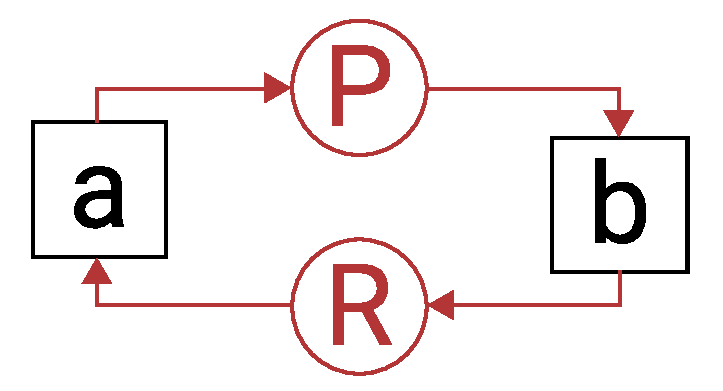
\includegraphics[scale=0.23]{gfx/theory/relationNode.pdf}}}
	\quad\Leftrightarrow\quad
	\exists\ a, b:\ {\color{rot}P(a, b) \land R(b, a)} \numberthis
\end{align*}

\paragraph{Negationskontexte (\textit{negation contexts} oder \textit{cuts})}
Für die Negation von Aussagen werden in Konzeptgraphen sog.~Kontexte verwendet.
Sie lassen sich neben der Negation auch zur Modellierung anderer Zusammenhänge nutzen, diese werden hier allerdings ausgelassen, um den Vergleich mit der Prädikatenlogik zu ermöglichen.
\begin{align*}
	\vcenter{\hbox{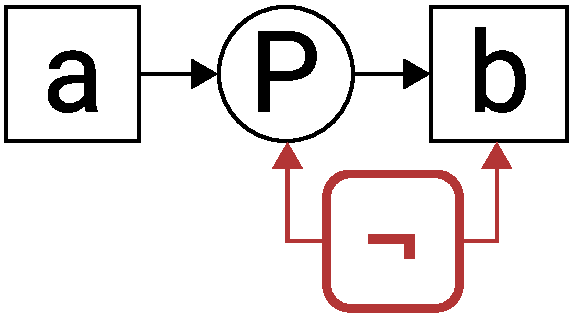
\includegraphics[scale=0.23]{gfx/theory/negationNode1.pdf}}}
	\quad\Leftrightarrow\quad
	&\exists\ a\ {\color{rot}\lnot\exists}\ b: P(a, b) \numberthis \\
	\quad\Leftrightarrow\quad
	&\exists\ a\ {\color{rot}\forall}\ b: {\color{rot}\lnot} P(a, b)
\end{align*}
Die Darstellung von Kontexten mit Knoten und Kanten wird schnell unübersichtlich, daher werden stattdessen Boxen verwendet, die die Kindknoten umschließen.
\begin{align*}
	\vcenter{\hbox{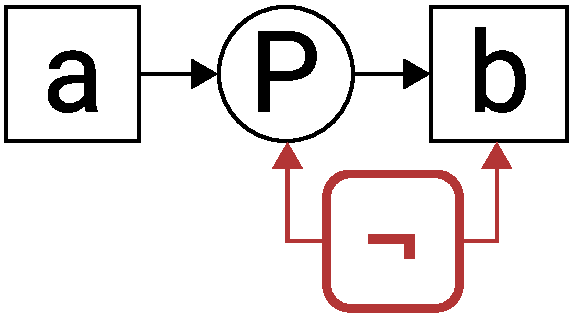
\includegraphics[scale=0.23]{gfx/theory/negationNode1.pdf}}}
	\quad\Leftrightarrow\quad
	\vcenter{\hbox{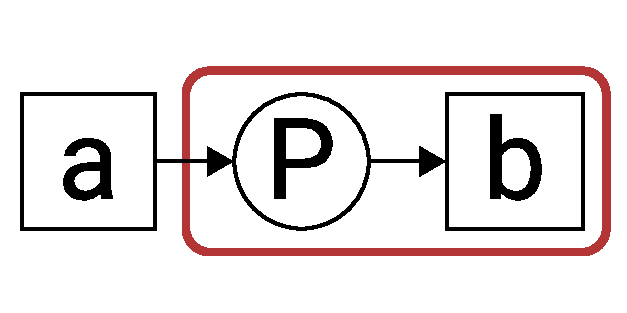
\includegraphics[scale=0.23]{gfx/theory/negationNode2.pdf}}}
\end{align*}
Kontexte können nicht nur Konzeptknoten und Relationsknoten enthalten, sondern auch andere Kontexte.
Hierbei ist zu beachten, dass alle Knoten und Kontexte höchstens einen Elternkontext haben können;
die Linien zweier Kontextboxen dürfen sich also nicht schneiden.
\begin{align*}
	\vcenter{\hbox{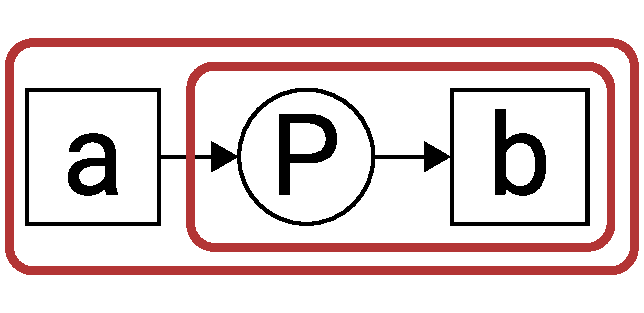
\includegraphics[scale=0.23]{gfx/theory/negationNode3.pdf}}}
	\quad\Leftrightarrow\quad
	&{\color{rot}\lnot\exists}\ a\ {\color{rot}\lnot\exists}\ b: P(a, b) \numberthis \\
	\quad\Leftrightarrow\quad
	&{\color{rot}\forall}\ a\ \exists\ b: P(a, b)
\end{align*}
\begin{align*}
	\vcenter{\hbox{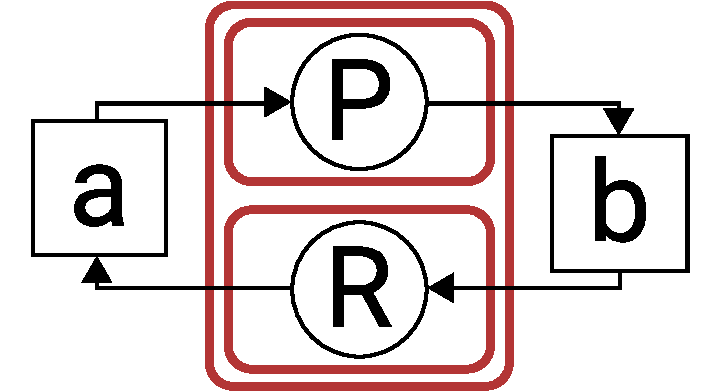
\includegraphics[scale=0.23]{gfx/theory/negationNode4.pdf}}}
	\quad\Leftrightarrow\quad
	&\exists\ a, b: {\color{rot}\lnot}({\color{rot}\lnot} P(a, b) \land {\color{rot}\lnot} R(b, a)) \numberthis \\
	\quad\Leftrightarrow\quad
	&\exists\ a, b: P(a, b)\ {\color{rot}\lor}\ R(b, a)
\end{align*}

\paragraph{Koreferenzkanten (\textit{coreference links})}
Entspricht der Äquivalenzrelation.
\begin{align}
	\vcenter{\hbox{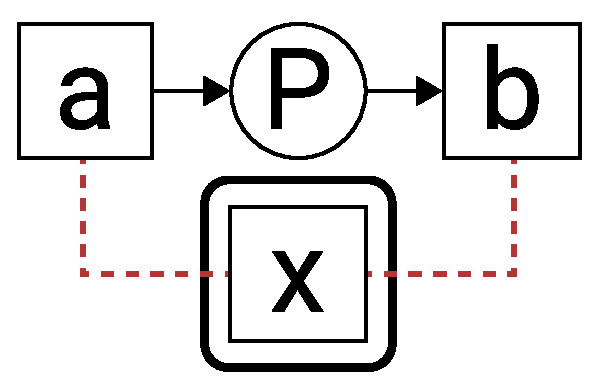
\includegraphics[scale=0.23]{gfx/theory/coreferenceEdge.pdf}}}
	\quad\Leftrightarrow\quad
	&\exists\ a, b: P(a, b) \land \lnot\exists\ x: {\color{rot}a = x \land x = b} \\
	\quad\Leftrightarrow\quad
	&\exists\ a, b: P(a, b) \land {\color{rot}a \neq b} \nonumber
\end{align}
Prinzipiell ließe sich die Äquivalenz auch durch Relationsknoten ausdrücken.
Um syntaktisch zu kennzeichnen, dass es sich nicht um eine beliebige Relation, sondern um eine Äquivalenzrelation handelt, wird dies jedoch i.~d.~R. nicht getan.
Koreferenzkanten können also als eine Kurzschreibweise verstanden werden, die den Zweck hat die für die Inferenz relevanten Symmetrie-, Transitivitäts- und Reflexivitätseigenschaften zu kennzeichnen.
\begin{align*}
	\vcenter{\hbox{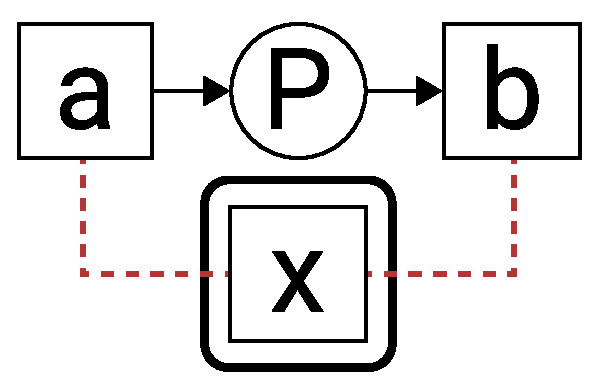
\includegraphics[scale=0.23]{gfx/theory/coreferenceEdge.pdf}}}
	\quad\Leftrightarrow\quad
	\vcenter{\hbox{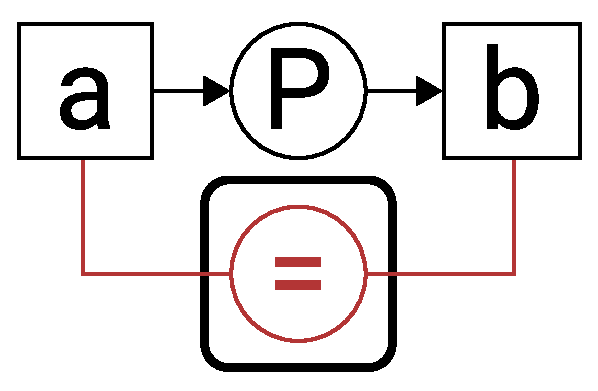
\includegraphics[scale=0.23]{gfx/theory/coreferenceEdgeAlternative.pdf}}}
\end{align*}

\subsection{Dominierende Knoten}%
\label{sec:theory:cg:domnodes}

So wie die Syntaxelemente prädikatenlogischer Ausdrücke nicht beliebig kombiniert werden können, unterliegen auch Konzeptgraphen gewissen Einschränkungen.
Die Einschränkung, dass alle Knoten und Kontexte höchstens einen Elternkontext haben dürfen, wurde bereits erwähnt.
Die zweite wichtige Einschränkung ist das Verbot nicht dominierender Knoten (\textit{dominating nodes}).
Was genau dies bedeutet, wird im Folgenden erläutert. Zuerst müssen Konzeptgraphen jedoch formal spezifiziert werden.
\begin{align*}
	G :=\ &(V, E) \text{, mit globalem Kontext } \top \in V \\
	concept(v) :\Leftrightarrow\ &\text{$v \in V$ ist ein Konzeptknoten} \\
	relation(v) :\Leftrightarrow\ &\text{$v \in V$ ist ein Relationsknoten} \\
	context(v) :\Leftrightarrow\ &\text{$v \in V$ ist ein Kontext, es gilt $context(\top)$} \\
	neg(v) :\Leftrightarrow\ &\text{$v \in V$ ist ein Negationskontext} \displaybreak[0]\\
	nest(c, v) :\Leftrightarrow\ &context(c) \land (c, v) \in E \\
	coref(v_1, v_2) :\Leftrightarrow\ &concept(v_1) \land concept(v_2) \land (v_1, v_2) \in E \\
	arg(r, v) :\Leftrightarrow\ &relation(r) \land concept(v) \land ((r, v) \in E \lor (v, r) \in E) \\ % chktex 35
	E \supseteq\ &\{ (\top, v): v \in V \land \lnot\exists\ c \in V \setminus \{ \top \}: nest(c, v) \} \displaybreak[0]\\
	a \leq b :\Leftrightarrow\ & (\exists\ x \in V: a \leq x \land x \leq b) \numberthis \\
	& \lor nest(b, a) \lor (\exists\ c \in V: nest(c, a) \land nest(c, b))
\end{align*}
Um die nachfolgenden Definitionen einfacher zu machen, wird der globale Kontext $\top$ eingeführt, der, in Anlehnung an Peirce, \textit{Sheet of Assertion} genannt wird.
$\top$ enthält alle Knoten, die keinen explizit dargestellten Elternkontext haben.
Die Kontextbox von $\top$ umschließt also den gesamten Konzeptgraphen.
$\leq$ ist eine Quasiordnung und bildet die \textit{enthalten-in}-Relation zwischen Knoten ab, d.~h.\ $a \leq b$ gdw.\ $a$ innerhalb der Box des Elternkontextes von $b$ liegt.
Das größte Element gemäß $\leq$ ist also immer $\top$.
\begin{figure}[h]
	\centering
	\[\vcenter{\hbox{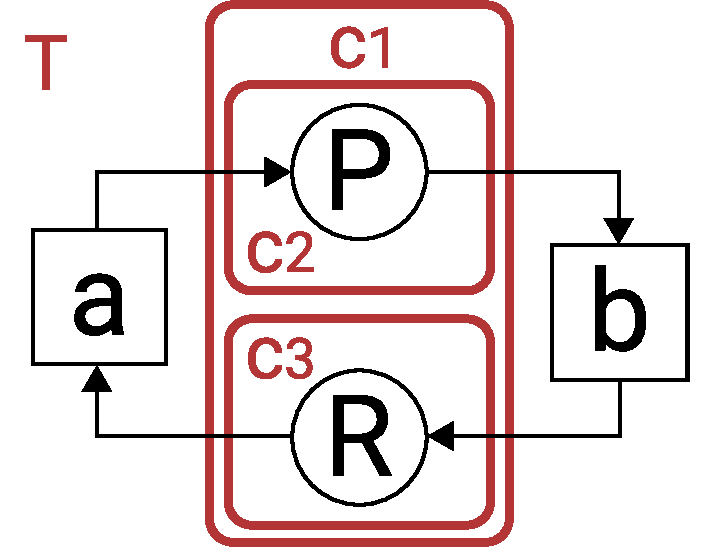
\includegraphics[scale=0.23]{gfx/theory/contextTreeExample1.pdf}}}
	\qquad
	\vcenter{\hbox{
		\begin{tikzpicture}[
			grow=down,
			sloped,
			level distance=2em,
			sibling distance=3em,
			edge from parent/.style={draw=black!70,latex-}]
			\node {\color{rot}$\top$}
				child {
					node (a) {$a$}
				}
				child {
					node (c1) {\color{rot}$c_1$}
						child {
							node (c2) {\color{rot}$c_2$}
								child {
									node {$P$}
								}
						}
						child {
							node (c3) {\color{rot}$c_3$}
								child {
									node {$R$}
								}
						}
				}
				child {
					node (b) {$b$}
				};
				\draw[latex-latex] (a) -- (c1);
				\draw[latex-latex] (c1) -- (b);
				\draw[latex-latex] (c2) -- (c3);
		\end{tikzpicture}
	}}\]
	\caption{Zusammenhang zwischen Kontexten und der $\leq$-Ordnung. Die Existenz eines Pfades von $x$ nach $y$ im obigen baumartigen Graphen, entspricht $x \leq y$.}\label{fig:theory:kgorder}
\end{figure}

Auf Basis von $\leq$ lässt sich nun das Konzept dominierender Knoten definieren.
\begin{align*}
	dom(G) :\Leftrightarrow\ & \forall\ r, v \in V: arg(r, v) \rightarrow r \leq v \numberthis \\ % chktex 35
	& \land \forall\ v_1, v_2 \in V: coref(v_1, v_2) \rightarrow (v_1 \leq v_2 \lor v_2 \leq v_1)
\end{align*}
Für jeden Konzeptgraphen $G$ muss $dom(G)$ gelten.
Eine Intuition für diese Einschränkung ist, dass es nicht sinnvoll ist die Existenz eines Atoms auszudrücken, welches durch nicht existente Variablen parametrisiert ist.
Eine detaillierte Untersuchung des Zwecks dominierender Knoten und eine Beschreibung der entstehenden Probleme, wenn auf die Notwendigkeit dominierender Knoten verzichtet wird, findet sich in~\cite[Abschnitt~14.3]{Dau2003}.
\begin{figure}[h]
	\begin{align*}
		\vcenter{\hbox{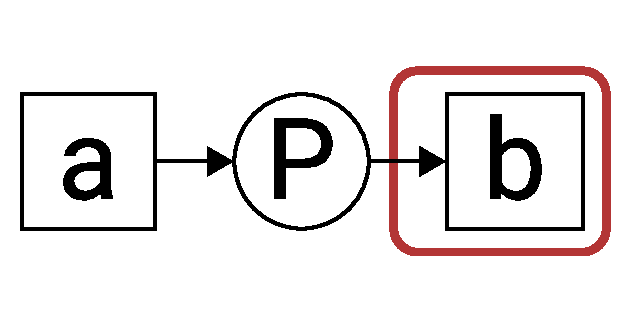
\includegraphics[scale=0.23]{gfx/theory/dominatingNodeViolation1.pdf}}}
		\quad
		&\text{\color{rot}$\lightning\ \lnot dom(G)$, da $arg(P, b) \land \lnot (P \leq b)$.} \\ % chktex 35
		\vcenter{\hbox{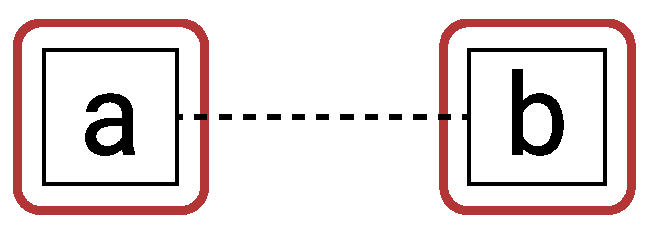
\includegraphics[scale=0.23]{gfx/theory/dominatingNodeViolation2.pdf}}}
		\quad
		&\text{\color{rot}$\lightning\ \lnot dom(G)$, da $coref(a, b) \land \lnot (a \leq b \lor b \leq a)$.}
	\end{align*}
	\caption{Beispiele für fehlerhafte Konzeptgraphen ohne dominierende Knoten.}\label{fig:theory:invalidkg}
\end{figure}

\section{Stanford CoreNLP}%
\label{sec:theory:nlp}

Um natürlichsprachliche Daten in einen Konzeptgraphen zu transformieren, ist im ersten Schritt eine Sprachanalyse notwendig.
Hierfür wurde die Stanford CoreNLP~\cite{CoreNLP} und die Apache OpenNLP~\cite{OpenNLP} Bibliothek in Erwägung gezogen, da beide häufig genutzt, aktiv weiterentwickelt, frei verfügbar und JVM-basiert sind.
Die JVM-Integration ist wichtig, um mit anderen verwendeten Bibliotheken kompatibel zu sein;
mehr hierzu in \treft{sec:text2kg:implementation}.
Für die Implementation wurde schließlich CoreNLP gewählt, da es mit den mitgelieferten Modellen häufig bessere Ergebnisse als OpenNLP liefert.
Da beide Bibliotheken bzgl.\ ihrer Funktionalität allerdings recht ähnlich sind, kann die NLP Komponente als substituierbar angesehen werden.
Ein Wechsel von CoreNLP auf OpenNLP wäre mit relativ geringem Aufwand möglich.

Im Folgenden wird nun die grundlegende Architektur von CorenNLP beschrieben.
CoreNLP verwendet das in~\ref{sec:related:nlp} vorgestellte Pipeline-Modell.
Die verschiedenen Verarbeitungsstufen der Pipeline werden Annotatoren genannt.
Da die genaue Funktionsweise der Annotatoren ist für diese Arbeit weniger relevant, wichtiger ist ein Überblick über die Art der Ergebnisse, die die Annotatoren liefern.

\paragraph{Tokenization und Lemmatization}
Liefern, wie erwartet, eine Liste von Token bzw.\ eine Liste der Lemmata der Token.
Es werden neben Englisch zahlreiche andere Sprachen und ein Großteil des Unicode Zeichensatzes unterstützt.
Der Tokenizer verwendet zum Finden der Tokens intern einen deterministischen endlichen Automaten.

\paragraph{POS-Tagging}
Ordnet jedem Token eine Wortart und Flexion (POS-Tag) zu.
Die Menge der möglichen POS-Tags wurde aus dem \textit{Penn Treebank Tag Set}~\cite{Santorini1990} übernommen.
Für das Finden der Tags benutzt CoreNLP sog.\ \textit{Cyclic Dependency Networks}~\cite{Toutanova2003}, eine Erweiterung bayesscher Netze, in denen zyklische Abhängigkeiten erlaubt sind.

\paragraph{Named Entity Recognition (NER)}
Findet sog.\ Entitäten.
CoreNLP benutzt hierfür eine Menge von Entitätsklassen, die sich in drei Kategorien von Klassen unterteilen lässt:
\begin{enumerate}
	\item \textbf{Benannte Entitäten:}
		Person, Ort, Organisation und Sonstige.
		Diese Entitätsklassen werden mittels \textit{Conditional Random Fields}~\cite{Finkel2005}, einer Variante von \textit{Markov Random Fields}~\tref{sec:theory:psl:mrf}, erkannt.
	\item \textbf{Numerische Entitäten:}
		Geldbetrag, Zahl, Ordinalzahl und Prozentzahl.
		Hierfür wird ein regelbasiertes System verwendet.
		Die so erkannten Token werden zudem normalisiert, um eine leichtere Weiterverarbeitung zu ermöglichen.
	\item \textbf{Temporale Entitäten:}
		Datum, Uhrzeit, Dauer und Menge von Zeitpunkten.
		Diese Klassen werden ebenfalls mit einem regelbasierten System erkannt.
		Mittels SUTime~\cite{Chang2012} werden die erkannten Token anschließend normalisiert und relative Zeitangaben in absolute Zeitpunkte aufgelöst, sofern ein Referenzzeitpunkt gegeben ist.
		Für die Normalisierung wird das TimeML TIMEX3-Format~\cite{TIMEX3} benutzt, mit dem sich auch komplexe Zeitangaben, wie \textit{``twice a week''} (\texttt{type=''set'' value=''P1W'' freq=''2X''}), formal ausdrücken lassen.
\end{enumerate}

\paragraph{Coreference Resolution}
Ermittelt Äquivalenzklassen von Token, die auf das selbe Konzept bzw.\ die selbe Entität verweisen.
CoreNLP stellt hierfür drei verschiedene Systeme bereit:
Ein schnelles, regelbasiertes, deterministisches System, ein etwas langsameres statistisches System und zuletzt ein langsames System, das auf neuronalen Netzen basiert.
Die langsameren Systeme liefern im Schnitt bessere Ergebnisse.

\paragraph{Dependency Parsing}
Dieser Annotator ermittelt die grammatikalischen Beziehungen zwischen Worten.
Das Ergebnis ist ein sog.\ Abhängigkeitsgraph (\textit{Dependency Graph}), in dem die Knoten Token und die Kanten Beziehungen repräsentieren.
CoreNLP verwendet für die Kantentypen \textit{Universal Dependencies Version 2} (UD v2)~\cite{UDv2}, eine Menge von 37 Arten grammatikalischer Beziehungen, die für eine vielzahl natürlicher Sprachen nutzbar ist.
Die Struktur der zurückgegebenen Abhängigkeitsgraphen, basiert auf einem ``\textit{{\color{blau}head}-{\color{rot}modifier}}''-Pattern;
d.~h.\ dass, ausgehend von einem \textit{\color{blau}head}-Token, Kanten zu \textit{\color{rot}modifier}-Token gehen, die die Bedeutug des \textit{\color{blau}heads} verändern.
\[
	\text{\color{rot}Peter's} \xleftarrow{\text{possessive nominal modifier}}
	\text{\color{blau}ball}
	\xrightarrow{\text{adjectival modifier}} \text{\color{rot}red}
\]
Der CoreNLP Dependency Parser nutzt ein sog.\ \textit{Transition-based Parsing}~\cite{Nivre2004}, bei dem alle Token der Reihe nach aus einem Buffer auf einen Stack von aktuell betrachteten Token gelegt werden.
Ein Klassifikator (im Falle von CoreNLP ist dies ein neuronales Netz) wählt dabei in jedem Schritt einen von drei Zustandsübergängen:
\begin{enumerate}
	\item \textbf{LEFT-ARC:}
		Fügt eine Abhängigkeitskante $(i, j)$ vom ersten Token $i$ des Stacks zum zweiten Token $j$ des Stacks ein und entfernt dann $j$ vom Stack.
	\item \textbf{RIGHT-ARC:}
		Fügt eine Abhängigkeitskante $(j, i)$ vom zweiten Token $j$ des Stacks zum ersten Token $i$ des Stacks ein und entfernt dann $i$ vom Stack.
	\item \textbf{SHIFT:}
		Verschiebt das erste Token des Buffers auf den Stack.
\end{enumerate}
Diese drei Zustandsübergänge werden so lange angewandt, bis der Buffer leer ist.
Durch die richtige Kombination von Übergängen lässt sich jeder beliebige Abhängigkeitsgraph beschreiben.

\section{Modellierung von HL-MRFs mit PSL}%
\label{sec:theory:psl}

In~\ref{sec:theory:cg} wurde beschrieben, wie komplexes Wissen durch Konzeptgraphen repräsentiert werden kann;
in~\ref{sec:theory:nlp} wurde beschrieben, wie der Inhalt natürlichsprachlicher Texte extrahiert und durch eine Menge von Abhängigkeiten repräsentiert werden kann.
Dieser Abschnitt beschreibt nun, wie aus einer Menge gegebenener Abhängigkeiten und Fakten neue Abhängigkeiten und Fakten inferiert werden können.
Konkrekt werden hierfür \textit{Hinge-Loss Markov Random Fields} (HL-MRFs) und die \textit{Probabilistic Soft Logic} (PSL) vorgestellt.

\subsection{Markov Random Fields}%
\label{sec:theory:psl:mrf}

MRFs sind, so wie auch bayessche Netze, eine Klasse von \textit{Probabilistischen Graphischen Modellen} (PGM);
d.~h.\ sie sind Graphen, deren Knoten als Zufallsvariablen und deren Kanten als stochastische Abhängigkeiten interpretiert werden.
Im Gegensatz zu bayesschen Netzen, sind die Kanten in MRFs allerdings ungerichtet, es sind also zyklische Abhängigkeiten erlaubt.
Formal beschreibt ein MRF $G$ die multivariate Verteilung $P$ eines Zufallsvektors $X$ gemäß einer Potentialfunktion $\Phi$:
\begin{align*}
	X :=&\ (X_1, \dots, X_n) = \text{Zufallsvektor} \\
	\mathcal{X} :=&\ \text{Menge aller möglichen Werte $(x_1, \dots, x_n)$ von $X$} \\
	G :=&\ (X, E) \\
	\mathcal{C} :=&\ \{ c_1, \dots, c_m \} = \text{Menge der maximalen Cliquen in $G$} \displaybreak[0]\\ % chktex 21
	X_c :=&\ \text{Vektor der Zufallsvariablen in der Clique $c \in \mathcal{C}$} \\
	\Phi_c(x_c) :=&\ \text{Cliquenpotential $\in \mathbb{R}^{+}_0$ der Werte $x_c$ von $X_c$} \\
	P(X = x) =&\ \frac{1}{Z} \prod_{i = 1}^{m} \Phi_{c_i}(x_{c_i}) \text{, mit Normalisierkonst.} Z := \sum_{x \in \mathcal{X}} \prod_{i = 1}^{m} \Phi_{c_i}(x_{c_i}) \numberthis
\end{align*}
Für MRFs gelten drei wichtige Eigenschaften bzgl.\ der Unabhängigkeit der Zufallsvariablen in $X$:
\begin{enumerate}
	\item \textbf{Globale Markov-Eigenschaft:}
		\[
			\forall X_A, X_B, X_S \subseteq X: sep_{X_A, X_B}(X_S) \rightarrow (X_A \perp X_B \mid X_S)
		\]
		Alle Paare $(X_A, X_B)$ von Teilmengen von $X$ sind bedingt unabhängig, sofern die Werte einer separierenden Teilmenge $X_S $ gegeben sind.
		$X_S$ ist separierend ($\Leftrightarrow sep_{X_A, X_B}(X_S)$), wenn alle Pfade von $a \in X_A$ nach $b \in X_B$ einen Knoten $s \in X_S$ enthalten.
	\item \textbf{Lokale Markov-Eigenschaft:}
		\[
			\forall X_i \in X: X_i \perp (X \setminus \Gamma(X_i) \setminus \{X_i\}) \mid \Gamma(X_i)
		\]
		Eine direkte Konsequenz der globalen Markov-Eigenschaft ist die lokale Markov-Eigenschaft.
		Jede Variable $X_i$ ist bedingt unabhängig von ihren nicht benachbarten Variablen, sofern ihre Nachbarschaft $\Gamma(X_i)$ gegeben ist.
	\item \textbf{Paarweise Markov-Eigenschaft:}
		\[
			\forall X_i, X_j \in X: \{X_i, X_j \} \notin E \rightarrow (X_i \perp X_j \mid X \setminus \{ X_i, X_j \})
		\]
		Aus der lokalen Markov-Eigenschaft folgt, dass jedes nicht adjazente Variablenpaar $(X_i, X_j)$ bedingt unabhängig voneinander ist, sofern alle anderen Variablen gegeben sind.
\end{enumerate}

\paragraph{Beispiel}
Die obigen Definitionen sind bislang noch recht abstrakt.
Ein exemplarisches praktisches Einsatzgebiet von MRFs ist das Lösen von SAT-Problemen.
Gegeben sei die SAT-Instanz ${\color{rot}(\lnot A \lor B \lor C)} \land {\color{blau}(\lnot C \lor \lnot D)}$.
MRFs können benutzt werden, um dieses Problem zu modellieren und eine erfüllende Belegung zu finden.\\
\begin{tabular}{m{0.25\textwidth} m{0.75\textwidth}}
	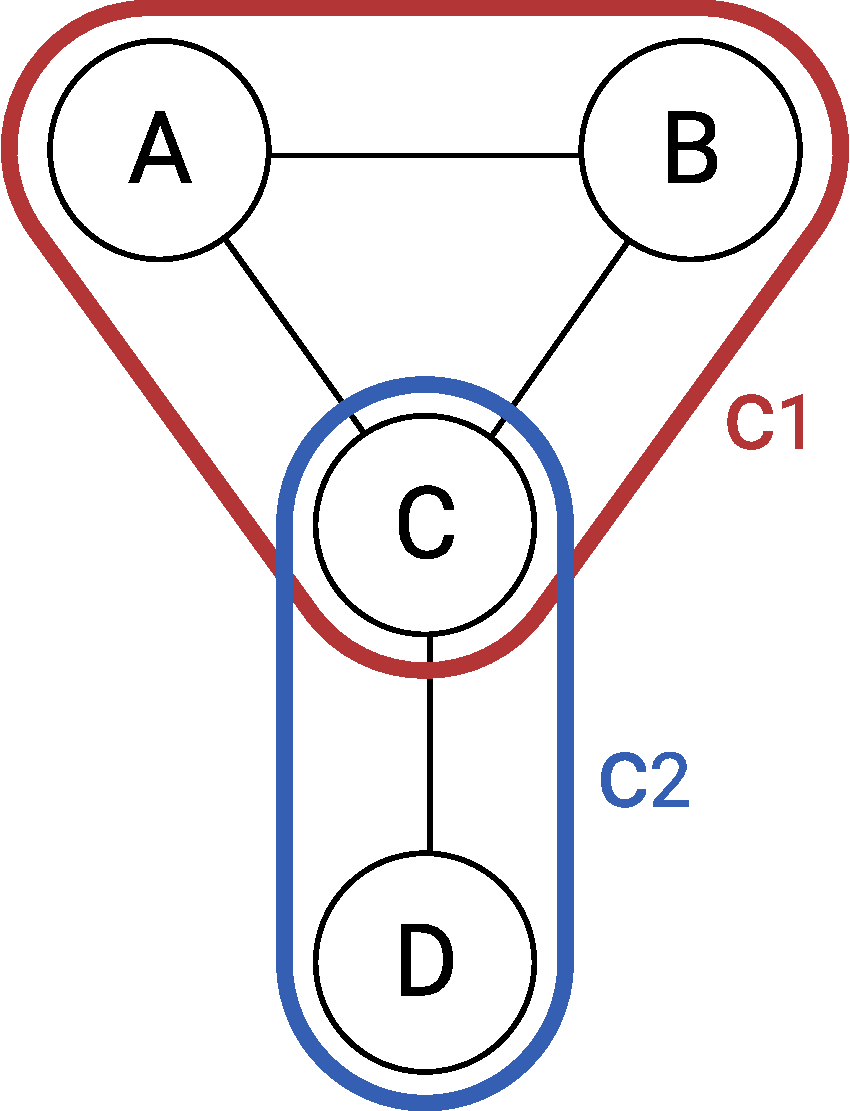
\includegraphics[width=0.23\textwidth]{gfx/theory/mrfExample1.pdf}
	&
	{\begin{align*}
		X :=&\ (A, B, C, D) \text{, mit } Bild(X) = {\{0, 1\}}^4 \\
		\mathcal{C} :=&\ \{{\color{rot}\underbrace{\{ A, B, C \}}_{c_1}}, {\color{blau}\underbrace{\{ C, D \}}_{c_2}}\} \\ % chktex 21
		{\color{rot}\Phi_{c_1}}(a, b, c) :=&\ \min\{ 1 - a + b + c, 1 \} \\ % chktex 21
		{\color{blau}\Phi_{c_2}}(c, d) :=&\ \min\{ 2 - c - d, 1 \} \\ % chktex 21
		P(X = (a, b, c, d)) :=&\ \frac{1}{Z} {\color{rot}\Phi_{c_1}}(a, b, c)\ {\color{blau}\Phi_{c_2}}(c, d)
	\end{align*}}
\end{tabular}\\
Eine Clique repräsentiert in diesem MRF eine Disjunktionsklausel und das Cliquenpotential gibt an, ob eine gegebene Belegung die Klausel erfüllt.
Gemäß dieser Definition, lässt sich die Erfüllbarkeit durch $\max_{x} P(X = x) > 0$ ausdrücken, d.~h.\ die Formel ist erfüllbar, gdw.\ es eine Variablenbelegung mit Eintrittswahrscheinlichkeit~$> 0$ gibt.
Die Normalisierungskonstante $Z$ hat auf das Ergebnis keinen Einfluss und kann daher ignoriert werden.

\paragraph{Das MRF-Inferenzproblem}
Da sich SAT, wie soeben exemplarisch gezeigt, auf MRFs reduzieren lässt, ist das Inferenzproblem, d.~h.\ das Finden einer maximal wahrscheinlichen Belegung der Zufallsvariablen, ein NP-schweres Problem.
Allgemeine, exakte und effiziente Lösungsalgorithmen existieren daher nicht.
Durch Einschränken der Struktur von $G$ und $\Phi$, oder durch das erlauben von Approximationen, lassen sich MRF-Inferenzen jedoch deutlich effizienter finden.
Wenn z.~B. $G$ ein Baum ist, kann mit dem \textit{Belief Propagation} Algorithmus eine exakte Lösung in polynomieller Zeit gefunden werden.

\subsection{Hinge-Loss MRFs}%
\label{sec:theory:psl:hlmrf}

Eine Unterart von MRFs, sind die sog.\ Hinge-Loss MRFs.
Sie sind so strukturiert, dass sich das Inferenzproblem effizient und exakt durch konvexe Optimierungsverfahren lösen lässt.
Es gibt drei wesentliche Unterschiede zu allgemeinen MRFs:
\begin{enumerate}
	\item
		Die Bedeutung von Zufallsvariablen und Kanten zwischen Zufallsvariablen ist klar definiert, da $\Phi$ nicht mehr frei wählbar ist.
		Ähnlich zum Beispiel aus~\ref{sec:theory:psl:mrf}, repräsentieren Zufallsvariablen aussagenlogische Variablen und Cliquen Disjunktionsklauseln.
	\item
		Für den Zufallsvektor $X$ muss $Bild(X) = {[0, 1]}^n$ gelten.
		Diese Einschränkung besteht, da jede HL-MRF-Zufallsvariable als die Wahrscheinlichkeit, dass eine aussagenlogische Variable wahr ist, interpretiert wird.
	\item
		Die Definition der Verteilung $P$ ist etwas anders:
		\begin{align*}
			P(X = x) :=&\ \frac{1}{Z} \prod_{i = 1}^{m} e^{w_i\,\Phi_i(x)} \propto \exp\left(\sum_{i=1}^{m} w_i\,\Phi_i(x)\right) = \exp\left(w\,{\Phi(x)}^\top\right) \numberthis \\
			w :=&\ (w_1, \dots, w_m) \in {[0, \infty]}^m,\ \Phi := (\Phi_1, \dots, \Phi_m)
		\end{align*}
		Auf die Cliquenpotentiale $\Phi_i$ wird nun die Exponentialfunktion angewandt, zudem erhalten alle Cliquen bzw.\ Klauseln $c_i$ ein Gewicht $w_i$.
		Das Inferenzproblem $\arg\max_{x} P(X = x)$ ist somit äquivalent zu $\arg\max_{x} w\,{\Phi(x)}^\top$.
\end{enumerate}

\paragraph{KNF-Formel Interpretation}
Aufgrund der Einschränkung von HL-MRFs auf aussagenlogische Ausdrücke, wird im Folgenden die Graphterminologie fallen gelassen und stattdessen die entsprechende aussagen\-logische Terminologie verwendet.
Ein HL-MRF wird nun als Repräsentation einer KNF-Formel $C_1 \land \dots \land C_m$ interpretiert.
Jede Disjunktionsklausel $C_j \in C$ wird durch eine Menge von Variablenindizes positiver Atome $I^{+}_j \subseteq \{1,\dots,n\}$ und eine Menge von Variablenindizes negativer Atome $I^{-}_j \subseteq \{1,\dots,n\}$ beschrieben.
\[
	C_j \cong \left(\bigvee_{i \in I^{+}_j} X_i\right) \lor \left(\bigvee_{i \in I^{-}_j} \lnot X_i\right)
\]

\paragraph{Łukasiewicz Logik}
Da die Variablen der KNF-Formel, gemäß obiger Definition, Werte~$\in [0, 1]$ annehmen können, ist nun noch unklar, wie die Operatoren $\land$, $\lor$ und $\lnot$ funktionieren sollen.
HL-MRFs benutzen hierfür die sog.\ Łukasiewicz Logik aus der Klasse der T-Norm Fuzzy Logiken;
sie ist eine Erweiterung der booleschen Logik, d.~h.\ die Łukasiewicz Operatoren verhalten sich für die Extrema $0$ und $1$ so, wie die booleschen Operatoren, sind aber ebenfalls für alle dazwischen liegenden Eingabewerte definiert.
\begin{align}
	x_1 \land x_2 :=&\ \max\{ x_1 + x_2 - 1, 0 \} \\ % chktex 21
	x_1 \lor x_2 :=&\ \min\{ x_1 + x_2, 1 \} \\ % chktex 21
	\lnot x :=&\ 1 - x
\end{align}
\begin{figure}[h]
	\centering
	\begin{tikzpicture}
		\begin{axis}[
			title={$\land$},
			xlabel=$x_1$,
			ylabel=$x_2$,
			width=0.35\textwidth,
			colormap = {bluered}{color(0cm) = (blau); color(1cm) = (rot)}
		]
			\addplot3[
				mesh,
				samples=12,
				domain=0:1,
				domain y=0:1
			]{max(x + y - 1, 0)};
		\end{axis}
	\end{tikzpicture}
	\begin{tikzpicture}
		\begin{axis}[
			title={$\lor$},
			xlabel=$x_1$,
			ylabel=$x_2$,
			width=0.35\textwidth,
			colormap = {bluered}{color(0cm) = (blau); color(1cm) = (rot)}
		]
			\addplot3[
				mesh,
				samples=12,
				domain=0:1,
				domain y=0:1
			]{min(x + y, 1)};
		\end{axis}
	\end{tikzpicture}
	\begin{tikzpicture}
		\begin{axis}[
			title={$\lnot$},
			xlabel=$x$,
			width=0.35\textwidth,
			colormap = {bluered}{color(0cm) = (blau); color(1cm) = (rot)}
		]
			\addplot[
				surf,
				domain=0:1
			]{1 - x};
		\end{axis}
	\end{tikzpicture}
	\caption{Visualisierung der Łukasiewicz Operatoren $\land$, $\lor$ und $\lnot$.}\label{fig:theory:luklogic}
\end{figure}

Mittels der Łukasiewicz Logik können Disjuktionsklauseln $C_j \in C$ für eine gegebene Variablenbelegung $x$ nun Wahrheitswerte~$\in [0, 1]$ zugeordnet werden.
Dieser Wahrheitswert wird als Klauselpotential $\Phi_j(x)$ verwendet.
Das HL-MRF-Inferenzproblem für KNF-Formeln in Łukasiewicz Logik ist demnach
\begin{alignat*}{3}
	\operatorname*{arg\,max}_{x \in {[0, 1]}^n}& \sum_{C_j \in C} w_j &&\Phi_j(x) \\ % chktex 35
	= \operatorname*{arg\,max}_{x \in {[0, 1]}^n}& \sum_{C_j \in C} w_j &&\left(\left(\bigvee_{i \in I^{+}_j} x_i\right) \lor \left(\bigvee_{i \in I^{-}_j} \lnot x_i\right)\right) \displaybreak[0]\\ % chktex 35
	= \operatorname*{arg\,max}_{x \in {[0, 1]}^n}& \sum_{C_j \in C} w_j \min &&\left\{ \left(\sum_{i \in I^{+}_j} x_i\right) + \left(\sum_{i \in I^{-}_j} (1 - x_i)\right), 1 \right\} \numberthis % chktex 21, chktex 35
\end{alignat*}

Statt die Summe der Wahrheitswerte $\Phi_j(x)$ zu maximieren, kann alternativ auch die Summe der Distanzen zur Erfüllung $\ell_j(x)$, genannt \textit{Distance to Satisfaction}, minimiert werden;
es gilt $\ell_j(x) = 1 - \Phi_j(x)$.
Gemäß dieser Interpretation ist ein HL-MRF somit eine Menge von gewichteten Constraints $\ell_j(x) \leq 0$, für die eine Lösung mit möglichst wenigen Verletzungen gesucht wird.
Das Inferenzproblem ist also
\begin{align*}
	\operatorname*{arg\,min}_{x \in {[0, 1]}^n}& \sum_{C_j \in C} w_j \max \{ \ell_j(x), 0 \} \displaybreak[0]\\ % chktex 35
	= \operatorname*{arg\,min}_{x \in {[0, 1]}^n}& \sum_{C_j \in C} w_j \max \left\{ 1 - \left(\sum_{i \in I^{+}_j} x_i\right) - \left(\sum_{i \in I^{-}_j} (1 - x_i)\right), 0 \right\} \numberthis % chktex 21, chktex 35
\end{align*}

\begin{figure}[h]
	\centering
	\begin{tikzpicture}
		\begin{axis}[
			xlabel=$x_1$,
			ylabel=$x_2$,
			y dir=reverse,
			width=0.45\textwidth,
			colormap = {bluered}{color(0cm) = (blau); color(1cm) = (rot)}
		]
			\addplot3[
				mesh,
				samples=20,
				domain=0:1,
				domain y=0:1
			]{max(1 - x - y, 0)};
		\end{axis}
	\end{tikzpicture}
	\caption{Visualisierung der Loss-Funktion $\ell_j(x_1, x_2)$ für $C_j \cong X_1 \lor X_2$}\label{fig:theory:hingeloss}
\end{figure}
Wie \figreft{fig:theory:hingeloss} für den zwei-elementigen Klauselfall veranschaulicht, handelt es sich bei $\ell$ um eine Hinge-Loss Funktion.
Hierher rührt die Bezeichnung Hinge-Loss MRF.\@
Da Hinge-Loss Funktionen konvex sind und die Summe konvexer Funktionen ebenfalls konvex ist, handelt es sich bei der HL-MRF-Inferenz um ein konvexes Optimierungsproblem.
Es existieren also effiziente und exakte Lösungsalgorithmen.
Einer dieser Algorithmen ist das \textit{Alternating Direction Method of Multipliers} Verfahren (ADMM), es wird in~\ref{sec:theory:psl:inference} näher vorgestellt.

\paragraph{MAX-SAT Äquivalenz}
In~\ref{sec:theory:psl:mrf} wurden MRFs anhand des Beispiels der SAT-Instanz ${\color{rot}(\lnot A \lor B \lor C)} \land {\color{blau}(\lnot C \lor \lnot D)}$ veranschaulicht.
Diese KNF-Formel hat folgendes Inferenzproblem, wenn sie als HL-MRF repräsentiert wird:
\[
	\operatorname*{arg\,min}_{(a, b, c, d) \in {[0, 1]}^4} {\color{rot}w_1 \max\{a - b - c, 0\}} + {\color{blau}w_2 \max\{c + d - 1, 0\}} % chktex 21, chktex 35
\]
Da in der Verteilung $P$ von HL-MRFs die Exponentialfunktion auf die Potentiale angewandt wird, bewirkt eine unerfüllte Klausel mit $\Phi_j(x) = 0$ nicht, dass $P(X = x) = 0$.
Stattdessen ist $P(X = x)$ proportional zu der Summe der Wahrheitswerte der Klauseln.
Die HL-MRF-Inferenz beschreibt also nicht SAT, sondern eine Fuzzy-Logik-Entsprechung von MAX-SAT.\@
Ein wichtiger Unterschied zum booleschen MAX-SAT ist, dass Klauseln gewichtet sind;
das Erfüllen einer Klausel mit hohem Gewicht kann das Nicht-Erfüllen mehrerer anderer Klauseln mit niedrigem Gewicht ausgleichen.

\subsection{Probabilistic Soft Logic}%
\label{sec:theory:psl:psl}

Wie soeben beschrieben, sind HL-MRFs ein flexibles Werkzeug, um Probleme, die sich durch MAX-SAT ausdrücken lassen, zu lösen.
Der Schritt von einem konkreten domänenspezifischen Problem in eine Menge von Klauseln $C$ und einen Gewichtsvektor $w$ ist bislang allerdings noch unklar.
An dieser Stelle setzt die \textit{Probabilistic Soft Logic} (PSL) an.
PSL ist eine formale Sprache, um mit einer intuitiven Syntax Klassen von HL-MRFs zu beschreiben.

\subsubsection{PSL Syntax}
Die Syntax von PSL ist an die Prädikatenlogik angelehnt und besteht aus sieben Arten von Elementen:
\begin{enumerate}
	\item \textbf{Konstanten:}
		Repräsentieren konstante Werte, wie z.~B. Strings oder Zahlen.
		Werden für domänenspezifische Daten, wie z.~B. Namen benutzt.
	\item \textbf{Variablen:}
		Werden während einer Inferenz mit Konstanten belegt.
		PSL Variablen sind nicht zu verwechseln mit den Zufallsvariablen in MRFs.
	\item \textbf{Terme:}
		Ein Term ist entweder eine Konstante oder eine Variable.
	\item \textbf{Prädikate:}
		Entsprechen in etwa den prädikatenlogischen Prädikaten.
		Jedes PSL Prädikat hat einen eindeutigen Bezeichner und eine Signatur aus Konstantentypen.
		\[Person: \text{UUID},\quad Name: \text{UUID} \times \text{String}\]
	\item \textbf{Atome:}
		Ein Atom ist ein Prädikat der Arität $n$, kombiniert mit einem $n$-Tupel von Termen.
		Das Term-Tupel enthält die Argumente des Prädikates.
		Wenn alle Argumente Konstanten sind, spricht man von einem Grundatom (\textit{ground atom}). \\
		\[Person(x),\quad Name(x, \text{``Alice''})\] % chktex 32
	\item \textbf{Literale:}
		Ein Literal ist entweder ein Atom oder ein negiertes Atom. \\
		\[Name(x, \text{``Alice''}),\quad \lnot Name(x, \text{``Bob''})\] % chktex 32
	\item \textbf{Regeln:}
		Eine Regel ist eine gewichtete Disjunktionsklausel von Literalen.
		Die negativen Atome der Klausel bilden dabei den sog.\ Körper $B$ (\textit{body}), die positiven Atome den sog.\ Kopf $H$ (\textit{head}) der Regel.
		Die so zerlegte Disjunktionsklausel lässt sich als Implikationsregel interpretieren:
		\[
			\left(\bigvee_{b \in B} \lnot b\right) \lor \left(\bigvee_{h \in H} h\right) \Leftrightarrow \left(\bigwedge_{b \in B}  b\right) \rightarrow \left(\bigvee_{h \in H} h\right)
		\]
		Mit Implikationen lassen sich nun intuitiv Zusammenhänge zwischen Prädikaten modellieren.\\
		\[0.65: Person(x) \land Name(x, \text{``Alice''}) \rightarrow Female(x)\] % chktex 32, chktex 1
\end{enumerate}

Eine Menge von PSL-Regeln wird PSL-Programm genannt.
Als Input erwartet ein PSL-Programm $R$ eine sog.\ Basis $\mathcal{A}$.
Die Basis ist dabei eine Menge von Grundatomen, die während der Inferenz in Betracht gezogen werden sollen, und setzt sich aus zwei disjunkten Teilmengen $\mathbb{C} \mathbin{\dot\cup} \mathbb{O} = \mathcal{A}$ zusammen.
$\mathbb{C}$ ist die Menge der geschlossenen (\textit{closed}) Grundatome, d.~h.\ der Wahrheitswert~$\in [0, 1]$ dieser Atome ist bekannt.
$\mathbb{O}$ umfasst die offenen (\textit{open}) Grundatome, deren Wahrheitswert noch unbekannt ist und daher inferiert werden soll.

\paragraph{Beispiel}
Ein Anwendungsgebiet von PSL ist z.~B. die Modellierung sozialer Beziehungen.
Angenommen, es sollen Freundschaftsbeziehungen zwischen Personen inferiert werden.
Ein stark vereinfachtes PSL-Programm hierfür könnte so aussehen:
\begin{align*}
	0.4:&\ \lnot Friends(A, B) & \rulemark{rule:theory:prior} \\
	0.5:&\ Friends(A, B) \land Friends(B, C) \land A \neq C \rightarrow Friends(A, C) & \rulemark{rule:theory:trans} \\
	1:&\ Interest(A, X) \land Interest(B, X) \rightarrow Friends(A, B) & \rulemark{rule:theory:sim} \\
	\infty:&\ Friends(A, B) \rightarrow Friends(B, A) & \rulemark{rule:theory:sym} \\
	\infty:&\ \lnot Friends(A, A) & \rulemark{rule:theory:irref}
\end{align*}
In dieser Regelmenge sind fünf Annahmen über das Verhalten der \texttt{Friends}-Relation kodiert:
\begin{enumerate}[label=$(r_{\arabic*})$]
	\item bildet ab, dass zwei Personen a~priori nicht miteinander befreundet sind.
		Eine solche PSL-Regel, die, in Ermanglung weiteren Wissens, das Nichtvorhanden\-sein einer Relation postuliert, wird \textit{Prior} genannt.
	\item bildet die Transitivität der $Friends$-Relation ab.
		Zwei Personen mit einem gemeinsamen Freund, sind evtl.\ befreundet.
		Das Infix-Prädikat $\neq$ ist üblicherweise vordefiniert.
	\item bildet ab, dass Personen mit einem gemeinsamen Interesse eine höhere Wahrscheinlichkeit haben befreundet zu sein.
	\item bildet die Symmetrie der $Friends$-Relation ab.
		Im Gegensatz zu den anderen Regeln, ist $r_4$ ein sog.\ \textit{Constraint}, d.~h.\ sie hat ein Gewicht $w_4 = \infty$.
		Das Nichterfüllen von $r_4$ hat somit zur Folge, dass die gewichtete Distance to Satisfaction ebenfalls den Wert $\infty$ annimmt und durch die Erfüllung anderer Regeln nicht ausgeglichen werden kann.
		Es ist also garantiert, dass jede MAX-SAT Lösung $r_4$ einhält;
		d.~h. $Friends(A, B) = Friends(B, A)$.
	\item ist ein weiterer Constraint, der die Irreflexivität von $Friends$ erzwingt.
\end{enumerate}

Für das PSL-Programm $R = \{r_1, \dots, r_5\}$ sei nun folgender Input $\mathcal{A}$ gegeben:
\begin{align*}
	\mathbb{C} &= \left\{ % chktex 21
		\begin{aligned}
			{\color{rot}Interest}(\text{``Alice''}, \text{``Reading''}) &= 0.5,\ &{\color{rot}Interest}(\text{``Dave''}, \text{``Reading''}) &= 1, \\
			{\color{rot}Interest}(\text{``Alice''}, \text{``Skiing''}) &= 0.5,\ &{\color{rot}Interest}(\text{``Charlie''}, \text{``Skiing''}) &= 1, \\
			{\color{rot}Interest}(\text{``Bob''}, \text{``Tennis''}) &= 1,\ &{\color{rot}Interest}(\text{``Charlie''}, \text{``Tennis''}) &= 1, \\
			{\color{gruen}Friends}(\text{``Alice''}, \text{``Bob''}) &= 1
		\end{aligned}
	\right\} \\ % chktex 21
	\mathbb{O} &= \{{\color{blau}Friends}(x, y) =\ \textbf{?} : x, y \in \{\text{``Alice''}, \text{``Bob''}, \text{``Charlie''}, \text{``Dave''}\}\} \setminus \mathbb{C} % chktex 21
\end{align*}
Die Interessen der Personen und die Freundschaft zwischen Bob und Alice aus $\mathbb{C}$ werden als bekannt angenommen.
Die gesuchten Freundschaftsrelationen aus $\mathbb{O}$ sollen inferiert werden.
\begin{figure}[h]
	\centering
	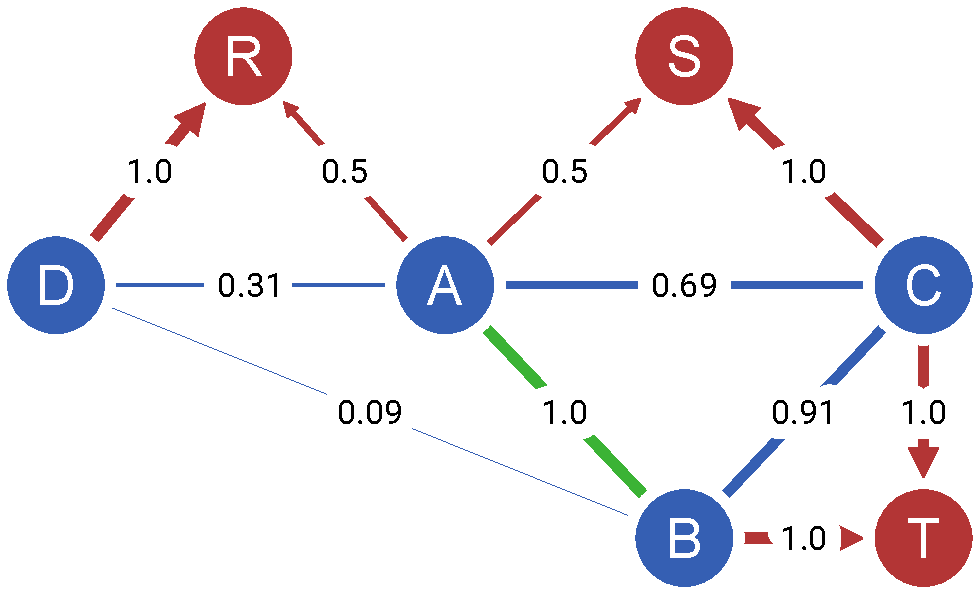
\includegraphics[width=0.6\textwidth]{gfx/theory/pslExample1.pdf}
	\caption{Graph der inferierten {\color{blau}$Friends$-Relation} und der gegebenen {\color{rot}$Interest$-Relation}.}\label{fig:theory:pslExample1}
\end{figure}
\figreft{fig:theory:pslExample1} zeigt ein mögliches MAX-SAT Ergebnis der Inferenz.
Wegen des Priors $r_1$ werden Personen generell als nicht befreundet eingeordnet.
Personen mit gemeinsamen Interessen werden hingegen, aufgrund von $r_3$, als Freunde erkannt.
Die durch $r_2$ modellierte Transitivitäteigenschaft ist ein weiterer verstärkender Faktor.
Dies lässt sich in der Clique \textit{Alice-Bob-Charlie} beobachten, die $Friends$-Beziehungen haben sich dort gegenseitig verstärkt.

\subsubsection{PSL~$\rightarrow$~HL-MRF Übersetzung}

Wie soeben gezeigt, ist PSL ein intuitiver Formalismus zur Definition relationaler Modelle.
Um Inferenzen durchzuführen, ist allerdings zuerst eine Übersetzung in ein HL-MRF notwendig.
Gegeben ist hierbei immer ein PSL-Programm $R = \{r_1, \dots, r_k\}$ und eine Eingabe $\mathcal{A} = \mathbb{C} \mathbin{\dot\cup} \mathbb{O}$.
Die Übersetzung erfolgt in zwei Schritten:
\begin{enumerate}
	\item \textbf{Zufallsvariablen:}
		Die Grundatome aus $\mathbb{C}$ werden zu Zufallsvariablen $X$, deren Belegung $x$ gegeben ist.
		Die Grundatome aus $\mathbb{O}$ werden zu Zufallsvariablen $Y$, für die die optimale Belegung $y \in \mathcal{Y}$ aus der Menge aller möglichen Belegungen $\mathcal{Y}$ gesucht wird.
		Der Zufallsvektor des HL-MRFs ist also $X \cup Y$.
	\item \textbf{Disjunktionsklauseln:}
		In der bisherigen HL-MRF Definition wurde stets davon ausgegangen, dass die optimale Belegung \textit{aller} Zufallsvariablen gesucht ist.
		Im Falle von PSL ist allerdings bereits bekannt, dass $X = x$ gilt.
		Das Inferenzproblem lautet daher wie folgt:
		\begin{align*}
			\operatorname*{arg\,max}_{y \in \mathcal{Y}} P(Y = y \mid X = x) =&\ \operatorname*{arg\,max}_{y \in \mathcal{Y}} P(X \cup Y = x \cup y) \numberthis \\ % chktex 35
			=&\ \operatorname*{arg\,max}_{y \in \mathcal{Y}} w\,{\Phi(y, x)}^\top % chktex 35
		\end{align*}
		Um ein HL-MRF zu erhalten, muss nun $\Phi$ und $w$, d.~h.\ die Menge der Klauseln $C$ und ihre Gewichte, definiert werden.
		Die PSL-Regeln in $R$ sind zwar Klauseln, können aber nicht direkt als $C$ verwendet werden, da sie potentiell freie PSL-Variablen enthalten, die PSL-Atome also potentiell nicht in $\mathcal{A}$ sind.
		Es erfolgt daher ein sog.\ \textit{Grounding} der PSL-Regeln.
		In jede Regel aus $R$ wird dabei jede mögliche Belegung der PSL-Variablen eingesetzt, sodass die resultierende Regelinstanz nur Atome aus $\mathcal{A}$ enthält.
		Die Menge dieser Regelinstanzen wird Grundregeln (\textit{ground rules}) genannt und als Klauselmenge $C$ benutzt.
		Aus $C$ wiederum lässt sich $\Phi$ nun mittels der Łukasiewicz Logik eindeutig ableiten.
		Das Gewicht jedes Potentials $\Phi_i$ ist dabei gleich dem Gewicht der PSL-Regel aus der es resultierte.
\end{enumerate}

\subsection{Inferenzverfahren}%
\label{sec:theory:psl:inference}

In \treft{sec:theory:psl:hlmrf} wurde die Konvexität des HL-MRF-Inferenzproblems bereits diskutiert.
Prinzipiell kann daher jedes konvexe Optimierungsverfahren im Kontext von HL-MRFs verwendet werden.
In der Praxis hat sich jedoch ein Verfahren, als besonders effizient erwiesen.

\paragraph{ADMM}
Das sog.\ \textit{Alternating Direction Method of Multipliers} Verfahren (ADMM) ist eine Variante des \textit{Method of Multipliers} Verfahrens, in der die dualen Variablen partiell aktualisiert werden.
Durch diese Variation lässt sich ADMM gut parallelisieren und ist somit geeignet für große Datenmengen und den Einsatz in Cluster-Umgebungen.
Das ursprüngliche Paper~\cite[Kapitel 10]{Boyd2011} beschreibt explizit, wie sich ADMM mit verteilten Datensets und verteilten Programmiermodellen wie z.~B. \textit{Map-Reduce} oder \textit{Pregel} implementieren lässt.

Die ADMM-Laufzeit ist proportional zur Klauselanzahl $|C|$.
Die Klauselanzahl wiederum wächst gemäß $\mathcal{O}(|\mathcal{A}|^r)$, wobei $r$ die maximale Anzahl von Nicht-Grund-Atomen in einer PSL-Regel ist.
Insgesamt wächst die Inferenzdauer also polynomiell in Abhängigkeit zur Eingabe $\mathcal{A}$.

\paragraph{BOCI}
Um effiziente Updates eines gegebenen Inferenzergebnises für eine veränderte Eingabe $\mathcal{A'}$ zu ermöglichen, wurde das \textit{Budgeted Online Collective Inference} (BOCI) Verfahren entwickelt.
Wenn ein Inferenzergebnis für $\mathcal{A} = \mathbb{C} \mathbin{\dot\cup} \mathbb{O}$ existiert und anschließend die Wahrheitswerte für einen Teil der bislang offenen Atome aus $\mathbb{O}$ bekannt werden, muss mittels BOCI keine weitere vollständige Inferenz durchgeführt werden.

Die Grundidee dabei ist es Metadaten, die während der letzten ADMM-Inferenz angefallen sind, für eine Bewertung jedes Atoms zu benutzen.
Die Bewertungen spiegeln die Volatilität der Wahrheitswerte der Atome, in Abhängigkeit von $\mathbb{C}$, wider.
Welche Metadaten für die Bewertung verwendet werden sollten, hängt stark von der Semantik der Wahrheitswerte der PSL-Prädikate ab.
In~\cite[Kapitel 4]{Pujara2015} werden verschiedene mögliche Bewertungsverfahren beschrieben, für diese Arbeit sind jene allerdings nicht näher relevant.

Gegeben sei also eine Bewertung der Atome aus $\mathcal{A}$.
Werden nun die Wahrheitswerte bislang offener Atome aus $\mathbb{O}$ bekannt, müssen ausschließlich die $m$ höchstbewerteten Atome aus $\mathbb{C}$ neu inferiert werden, die Wahrheitswerte aller anderen Atome werden fixiert.
Je höher das sog.\ Budget $m$, desto höher ist die Qualität im Vergleich zu einer vollständigen Inferenz.
Es wurde empirisch gezeigt, dass die Inferenzqualität mit BOCI gegenüber einer vollständigen Inferenz meist nur unwesentlich schlechter ist, während sich die Inferenzdauer teils um über 60\% verringert~\cite[Kapitel 5]{Pujara2015}.
